\begin{Ponto}{M}
		\label{primeira_tabela_pM}
		\begin{PontoTabela}
			\fileName{CMS013.CMG}
			\fileInit{10/10/0016 10:00:10}
			\fileFim{10/10/0016 10:03:10}
			\fileInfo{59.94}{54.0}{76.4}{0.0}{0.0}
		\end{PontoTabela}
\end{Ponto}
Na \textbf{Figura \ref{primeiro_grafico_pM}} é apresentado o histórico no tempo do nível sonoro do \textbf{Ponto \ponto{M}}, não houve necessidade de tratamento estatístico porque o ruído representado durante a amostragem foi somente do ambiente. \\*
			\begin{figure}[H]
				\centering
				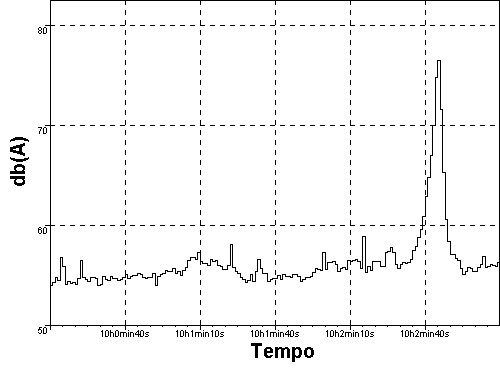
\includegraphics[width=8cm]{pontos/CMS013.PNG}
				\caption{Gráfico sem tratamento}
				\label{primeiro_grafico_pM}
			\end{figure}

\newpage
\begin{Ponto}{M}
		\begin{PontoTabela}
			\fileName{CMS014.CMG}
			\fileInit{10/10/0016 10:04:23}
			\fileFim{10/10/0016 10:07:23}
			\fileInfo{49.77}{45.1}{61.5}{0.0}{0.0}
		\end{PontoTabela}
\end{Ponto}
Na \textbf{Figura \ref{grafico_ref_12}} é apresentado o histórico no tempo do nível sonoro do \textbf{Ponto \ponto{M}}, não houve necessidade de tratamento estatístico porque o ruído representado durante a amostragem foi somente do ambiente. \\*
			\begin{figure}[H]
				\centering
				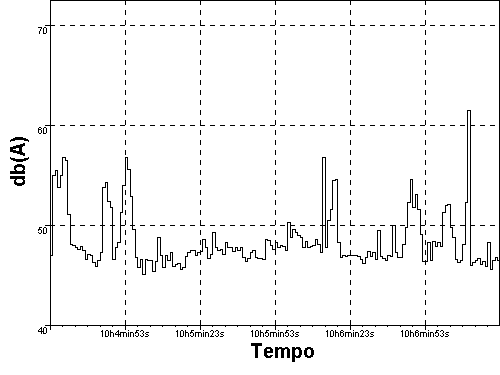
\includegraphics[width=8cm]{pontos/CMS014.PNG}
				\caption{Gráfico sem tratamento}
				\label{grafico_ref_12}
			\end{figure}

\newpage
\begin{Ponto}{M}
		\begin{PontoTabela}
			\fileName{CMS015.CMG}
			\fileInit{10/10/0016 10:10:07}
			\fileFim{10/10/0016 10:13:07}
			\fileInfo{50.51}{39.6}{56.5}{0.0}{0.0}
		\end{PontoTabela}
\end{Ponto}
Na \textbf{Figura \ref{grafico_ref_13}} é apresentado o histórico no tempo do nível sonoro do \textbf{Ponto \ponto{M}}, não houve necessidade de tratamento estatístico porque o ruído representado durante a amostragem foi somente do ambiente. \\*
			\begin{figure}[H]
				\centering
				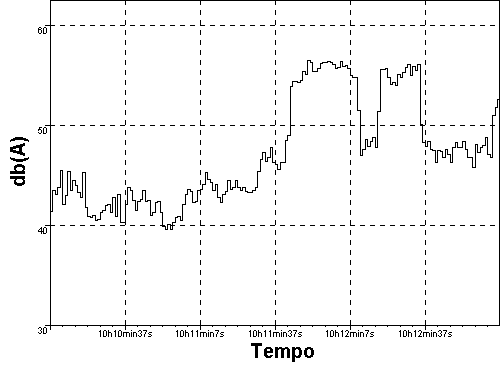
\includegraphics[width=8cm]{pontos/CMS015.PNG}
				\caption{Gráfico sem tratamento}
				\label{grafico_ref_13}
			\end{figure}

\newpage
\begin{Ponto}{M}
		\begin{PontoTabela}
			\fileName{CMS016.CMG}
			\fileInit{10/10/0016 10:16:11}
			\fileFim{10/10/0016 10:19:11}
			\fileInfo{55.43}{35.6}{71.8}{0.0}{0.0}
		\end{PontoTabela}
\end{Ponto}
Na \textbf{Figura \ref{grafico_ref_14}} é apresentado o histórico no tempo do nível sonoro do \textbf{Ponto \ponto{M}}, não houve necessidade de tratamento estatístico porque o ruído representado durante a amostragem foi somente do ambiente. \\*
			\begin{figure}[H]
				\centering
				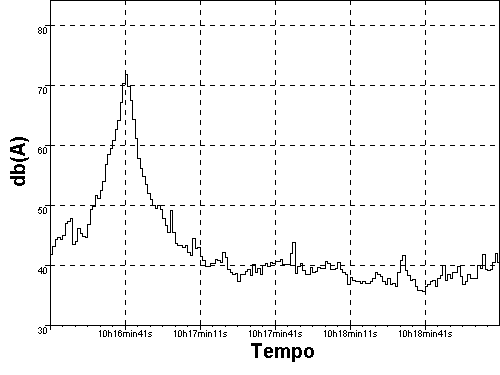
\includegraphics[width=8cm]{pontos/CMS016.PNG}
				\caption{Gráfico sem tratamento}
				\label{grafico_ref_14}
			\end{figure}

\newpage
\begin{Ponto}{M}
		\label{ultima_tabela_pM}
		\begin{PontoTabela}
			\fileName{CMS017.CMG}
			\fileInit{10/10/0016 10:20:31}
			\fileFim{10/10/0016 10:23:31}
			\fileInfo{55.3}{37.5}{61.9}{0.0}{0.0}
		\end{PontoTabela}
\end{Ponto}
Na \textbf{Figura \ref{ultimo_grafico_pM}} é apresentado o histórico no tempo do nível sonoro do \textbf{Ponto \ponto{M}}, não houve necessidade de tratamento estatístico porque o ruído representado durante a amostragem foi somente do ambiente. \\*
			\begin{figure}[H]
				\centering
				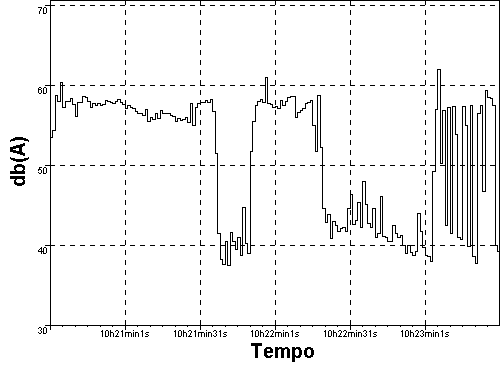
\includegraphics[width=8cm]{pontos/CMS017.PNG}
				\caption{Gráfico sem tratamento}
				\label{ultimo_grafico_pM}
			\end{figure}

\newpage
